\textbf{\underline{OZ 1 - Herhaling - Oefening 2:}}
\vspace{0.5cm}

\textbf{Regels van Kirchhoff:} Bepaal de groottes en de richtingen van de stromen door elke weerstand in Figuur 1.1 voor (a) geen interne weerstand in de batterij en (b) een interne weerstand van $ r = 1.0 \Omega $ in beide batterijen. De batterijen hebben een emf van $ \epsilon_1 = 9.0 V $ en $ \epsilon_2 = 12.0 V $, en de weerstanden hebben een waarde van $ R_1 = 25 \Omega $, $ R_2 = 48 \Omega $ en $ R_3 = 35 \Omega $.

\begin{figure}[H]
    \centering
    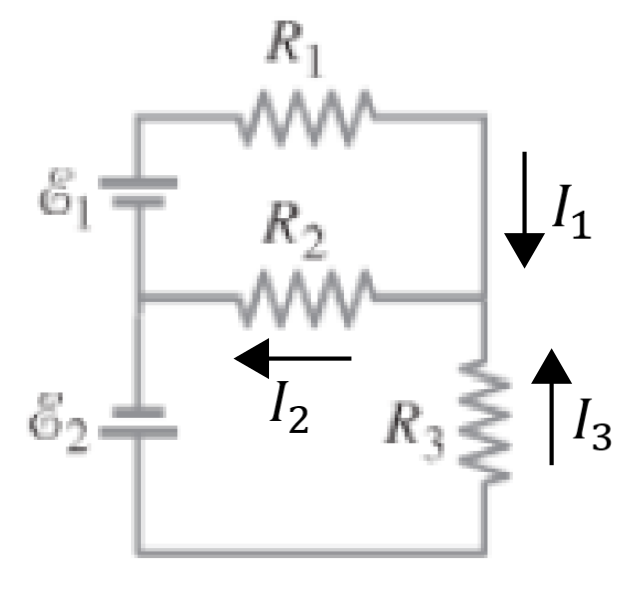
\includegraphics[width=3cm]{oz01/herhaling/resources/oef-2-opgave+schets.png}
    
    \textbf{Figuur 1.1}
\end{figure}

\begin{description}[labelwidth=1.5cm, leftmargin=!]
     \item[Geg. :]   $ r_1 = 0 \ \Omega $; $ r_2 = 1 \ \Omega $; $ \epsilon_1 = 9.0 $ V; $ \epsilon_2 = 12.0 $ V; $ R_1 = 25 \ \Omega $; $ R_2 = 48 \ \Omega $; $ R_3 = 35\  \Omega $;
    \item[Gevr. :]  $ I_1 $; $ I_2 $; $ I_3 $;
    \item[Opl. :]   $ \left\{\begin{array}{l}
                        I_1 + I_3 = I_2 \\
                        r_1 \cdot I_1 + R_1 \cdot I_1 + R_2 \cdot I_2 = \epsilon_1 \\
                        r_2 \cdot I_3 + R_3 \cdot I_3 + R_2 \cdot I_2 = \epsilon_2
                    \end{array}\right. $
                    
                    \hspace{-0.57cm} $ \Leftrightarrow 
                    \left\{\begin{array}{l}
                        I_1 + I_3 = I_2 \\
                        0 \cdot I_1 + 25 \cdot I_1 + 48 \cdot I_2 = 9.0 \\
                        1 \cdot I_3 + 35 \cdot I_3 + 48 \cdot I_2 = 12.0
                    \end{array}\right. $
                    
                    \hspace{-0.57cm} $ \Leftrightarrow 
                    \left\{\begin{array}{rcrcrcl}
                        I_1 & - & I_2 & + & I_3 & = & 0 \\
                        25 \cdot I_1 & + & 48 \cdot I_2 & & & = & 9.0 \\
                        & & 48 \cdot I_2 & + & 36 \cdot I_3 & = & 12.0
                    \end{array}\right. $
                    
                    \hspace{-0.57cm} $ \Rightarrow 
                    \left(\begin{array}{ccc|c}
                        1  & -1 & 1  & 0   \\
                        25 & 48 & 0  & 9.0 \\
                        0  & 48 & 36 & 12.0
                    \end{array}\right)
                    \xrightarrow{R_2 \to R_2 - 25 R_1} 
                    \left(\begin{array}{ccc|c}
                        1  & -1 & 1   & 0   \\
                        0  & 73 & -25 & 9.0 \\
                        0  & 48 & 36  & 12.0
                    \end{array}\right) $
                    
                    $ \xrightarrow{R_3 \to R_3 - \frac{48}{73} R_2} 
                    \left(\begin{array}{ccc|c}
                        1  & -1 & 1               & 0   \\
                        0  & 73 & -25             & 9.0 \\
                        0  & 0  & \frac{3828}{73} & \frac{444}{73}
                    \end{array}\right)
                    \xrightarrow{R_3 \to \frac{73}{3828} R_3} 
                    \left(\begin{array}{ccc|c}
                        1  & -1 & 1   & 0   \\
                        0  & 73 & -25 & 9.0 \\
                        0  & 0  & 1   & \frac{111}{957}
                    \end{array}\right)$
                    
                    \hspace{-0.57cm} $ \Rightarrow 
                    \left\{\begin{array}{l}
                        I_1 - I_2 + I_3 = 0 \\
                        73 \cdot I_2 - 25 \cdot I_3 = 9.0 \\
                        I_3 = \frac{111}{957} \ \textrm{A} \approx 0.12 \ \textrm{A}
                    \end{array}\right. $
                    
                    \hspace{-0.57cm} $ \Leftrightarrow 
                    \left\{\def\arraystretch{1.3}\begin{array}{l}
                        I_1 = I_2 - \frac{111}{957} \\
                        I_2 = \frac{9.0 + 25 \cdot I_3}{73} = \frac{9.0 + 25 \cdot \frac{111}{957}}{73} = \frac{52}{319} \ \textrm{A} \approx 0.16 \ \textrm{A} \\
                        I_3 = \frac{111}{957} \ \textrm{A} \approx 0.12 \ \textrm{A}
                    \end{array}\right. $
                    
                    \hspace{-0.57cm} $ \Leftrightarrow 
                    \left\{\def\arraystretch{1.3}\begin{array}{l}
                        I_1 = \frac{52}{319} - \frac{111}{957} = \frac{15}{319} \ \textrm{A} \approx 0.047 \ \textrm{A} \\
                        I_2 = \frac{9.0 + 25 \cdot I_3}{73} = \frac{9.0 + 25 \cdot \frac{111}{957}}{73} = \frac{52}{319} \ \textrm{A} \approx 0.16 \ \textrm{A} \\
                        I_3 = \frac{111}{957} \ \textrm{A} \approx 0.12 \ \textrm{A}
                    \end{array}\right. $
\end{description}

\vspace{1cm}